\subsection{Обзор существующих аналогов}
\label{sec:analysis:analogues}

Для решения задач менеджмента персонала могут использоваться различные средства. Рассмотрим каждую из задач в
отдельности.

\subsubsection{} Управление кадрами
\label{sec:analysis:analogues:managment}

Прибыльная и стабильная деятельность любого предприятия в первую очередь зависит от правильно выбранного системного
подхода к рабочему коллективу. Для достижения наилучших результатов работы сотрудников были разработаны системы,
благодаря которым обеспечивается автоматизация управления персоналом. 

Данные системы состоят из набора мероприятий, целью проведения которых является организация эффективного руководства
работниками компании и соответственно достижение наилучшего качества управления кадровыми ресурсами. При наличии
необходимого количества профессиональных сотрудников в штате организации, автоматизированная система управления
персоналом гарантирует быстроту достижения бизнес-целей предприятия без дополнительных финансовых расходов.
Кроме этого, привлечение HR-менеджмента к рабочему процессу какой-либо компании позволяет:
\begin{itemize}
	\item повышать уровень продуктивной деятельности всего кадрового состава;
	\item значительно расширять клиентскую базу;
	\item увеличивать спрос на товары или услуги;
	\item сохранять целостность всех процессов в бизнесе;
	\item обеспечивать удовлетворенность клиентов.
\end{itemize}

Первой и самой основной функцией системы управления сотрудниками стало планирование персонала. Ее цель заключается в
тщательной разработке политики кадрового отдела и составление стратегического плана руководства рабочим составом
предприятия. Также в планирование персонала вошел профессиональный анализ потенциала работников, составление прогноза
потребностей в привлечении новых соискателей и поддержание связи с внешними источниками, которые помогают привлекать в
организацию новых кандидатов.

На втором месте стоит функция, отвечающая за оценку уровня знаний работников и обеспечение их дальнейшего развития.
В основном в этот процесс входит осуществление обучения новых сотрудников, переподготовка и повышение уровня
профессионализма всего рабочего коллектива в целом. Также специалисты отвечают за введение в должность и помогают
адаптироваться новичкам в кадровом составе. Кроме этого, функция оценки, обучения и развития сотрудников помогает
правильно организовывать мероприятия, позволяющие управлять карьерным ростом персонала.

На данный момент существует множество систем управления персоналом персоналом с широким набором возможностей. В
процессе проектирования системы были изучены следующие программные решения:
\begin{itemize}
	\item E-Staff;
	\item 1С:Зарплата и управление персоналом.
\end{itemize}

1.2.1.1 E-Staff

Система E-Staff существует на рынке с 2000 года. Система предназначена для HR-служб компаний, осуществляющих подбор
сотрудников, и для кадровых агентств. E-Staff -- система полного цикла, автоматизирующая большинство рутинных операций
в рекрутинге(рисунок \ref{fig:analysis:analogues:e-staff}).
\pagebreak

\begin{figure}
	\centering
	
\includegraphics[scale=0.5]{e-staff.png} 
	\caption{Стартовая страница E-Staff}
	\label{fig:analysis:analogues:e-staff}
\end{figure}

Структурные подразделения могут быть автоматически загружены из системы кадрового учета компании
(1С, БОСС-Кадровик, SAP и др.). Также их можно завести вручную, если бизнес-структура компании не совпадает с
формальной штатной структурой(рисунок \ref{fig:analysis:analogues:e-staff-departments}).

\begin{figure}[!h]
	\centering
	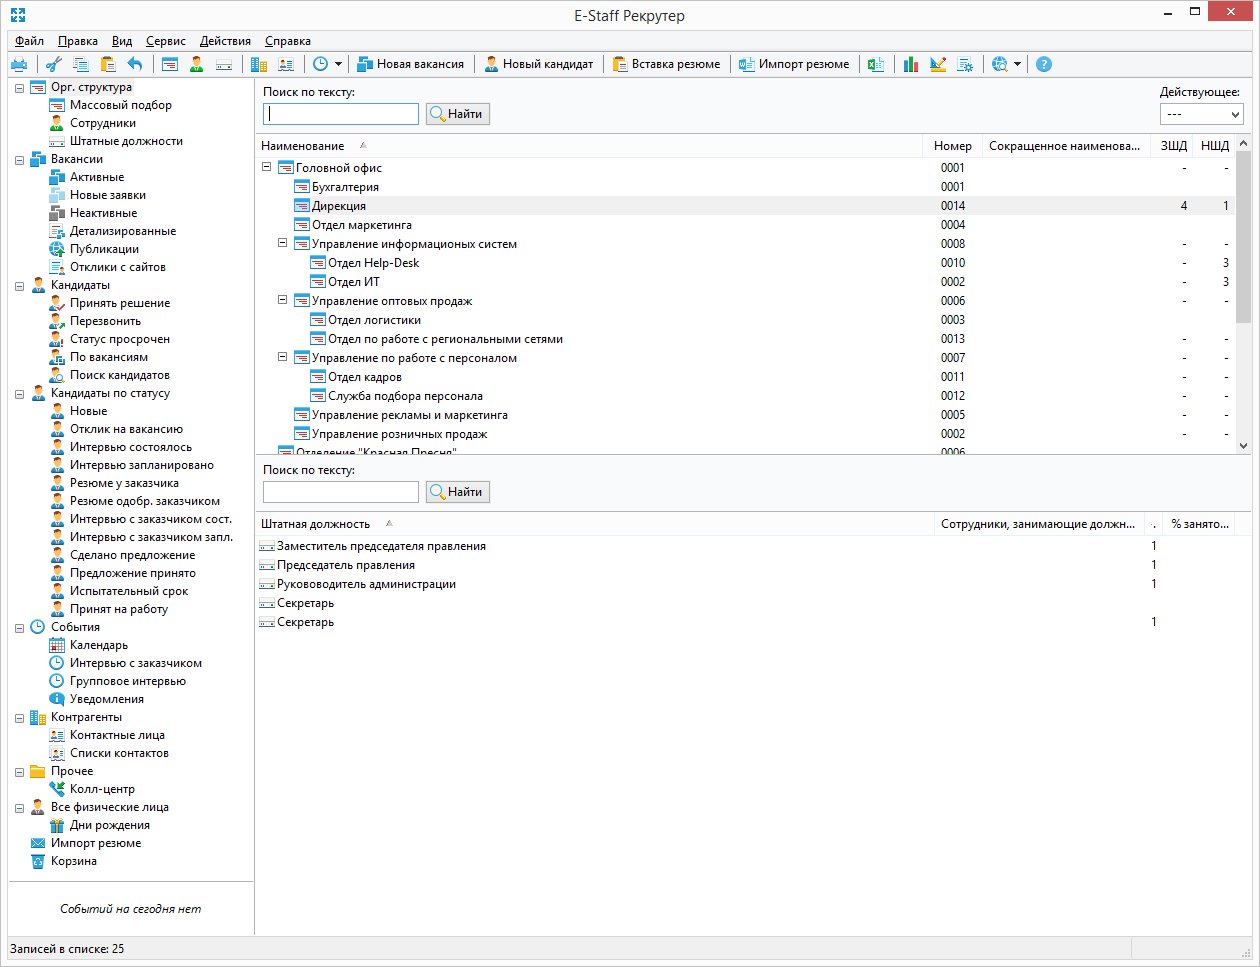
\includegraphics[scale=0.5]{e-staff-departments.png} 
	\caption{Управление подразделениями в системе E-Stuff}
	\label{fig:analysis:analogues:e-staff-departments}
\end{figure}

Также как и список подразделений, список сотрудников компании может автоматически синхронизироваться с системой
кадрового учета компании (1С, БОСС-Кадровик, SAP и др.) (рисунок \ref{fig:analysis:analogues:e-staff-employees}).

\begin{figure}[!h]
	\centering
	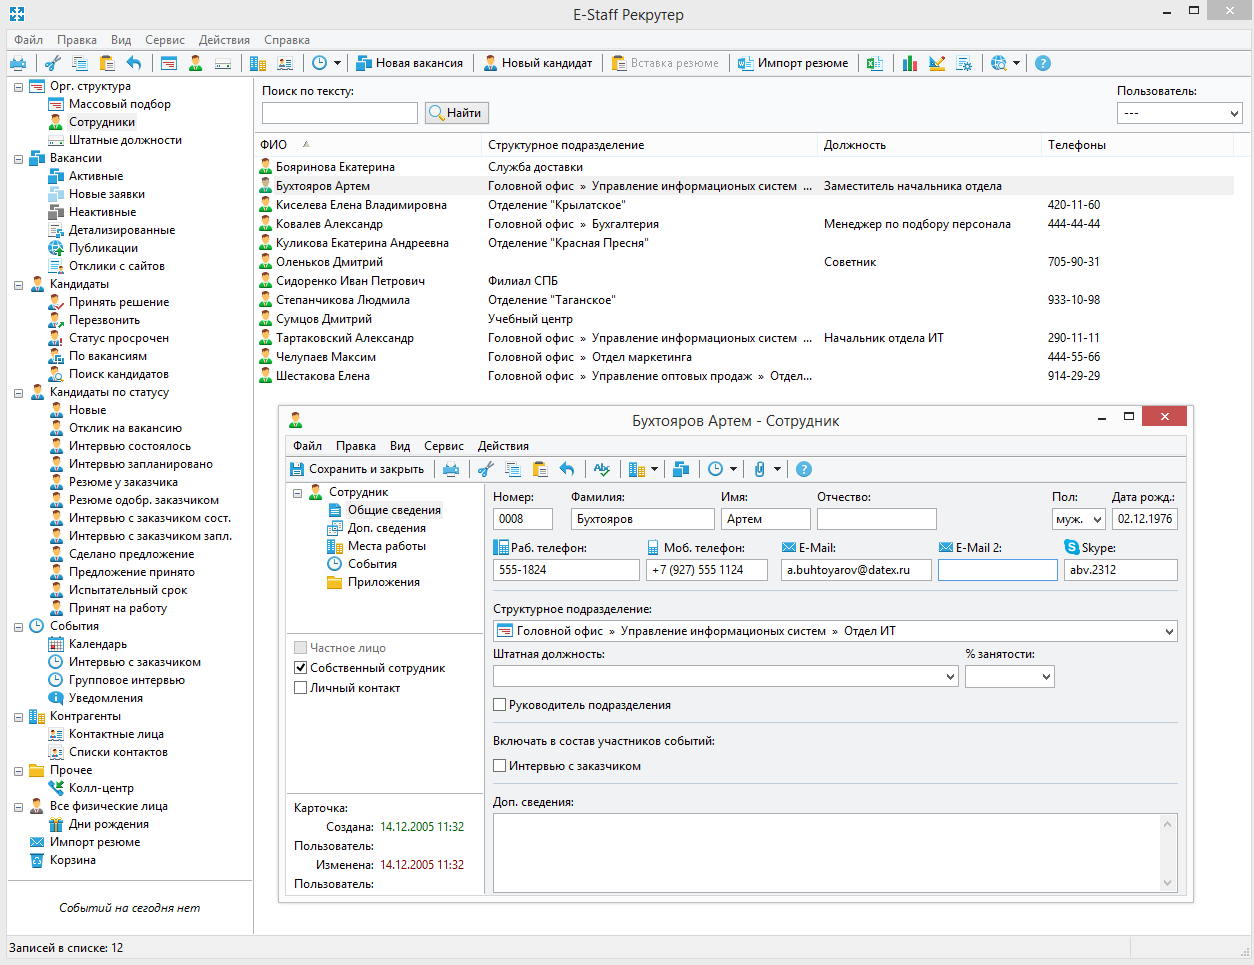
\includegraphics[scale=0.5]{e-staff-employees.png} 
	\caption{Управление сотрудниками в системе E-Stuff}
	\label{fig:analysis:analogues:e-staff-employees}
\end{figure}

Преимущества системы:
\begin{itemize}
	\item Хранение данных о структуре и сотрудниках компании;
	\item Работа с вакансиями компании;
	\item Импорт данных из сторонних систем;
	\item Поиск резюме в сети Интернет.
\end{itemize}

Недостатки системы:
\begin{itemize}
	\item ПО требует приобретения;
	\item Устаревший интерфейс;
	\item Отсутсвие кроссплатформенности.
\end{itemize}

1.2.1.2 1С:Зарплата и управление персоналом

1С:Зарплата и управление персоналом -- программа массового назначения, позволяющая в комплексе автоматизировать
задачи, связанные с расчетом заработной платы персонала и реализацией кадровой политики, с учетом требований
законодательства и реальной практики работы предприятий. Она может успешно применяться в службах управления персоналом
и бухгалтериях предприятий, а также в других подразделениях, заинтересованных в эффективной организации работы
сотрудников, для управления человеческими ресурсами коммерческих предприятий различного масштаба
(рисунок \ref{fig:analysis:analogues:1c}).

В 1С:Зарплате и управлении персоналом поддерживаются все основные процессы управления персоналом, а также процессы
кадрового учета, расчета зарплаты, исчисления налогов, формирования отчетов и справок в государственные органы и
социальные фонды, планирования расходов на оплату труда. Учтены требования законодательства, реальная практика работы
предприятий и перспективные мировые тенденции развития подходов к управлению персоналом.

Кадровый учет обязателен для любой компании. С каждым годом он все более регламентируется законодательством, поэтому
возможность его автоматизации важна для многих компаний, особенно с большим штатом сотрудников
(рисунок \ref{fig:analysis:analogues:1c_employees}).

\begin{figure}[!h]
	\centering
	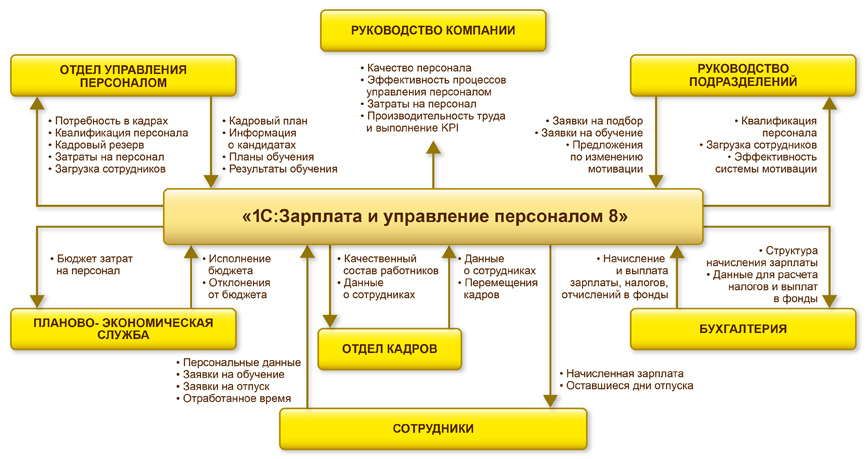
\includegraphics[scale=0.5]{1c.jpg} 
	\caption{Основные функции системы 1С:Зарплата и управление персоналом}
	\label{fig:analysis:analogues:1c}
\end{figure}

\begin{figure}[!h]
	\centering
	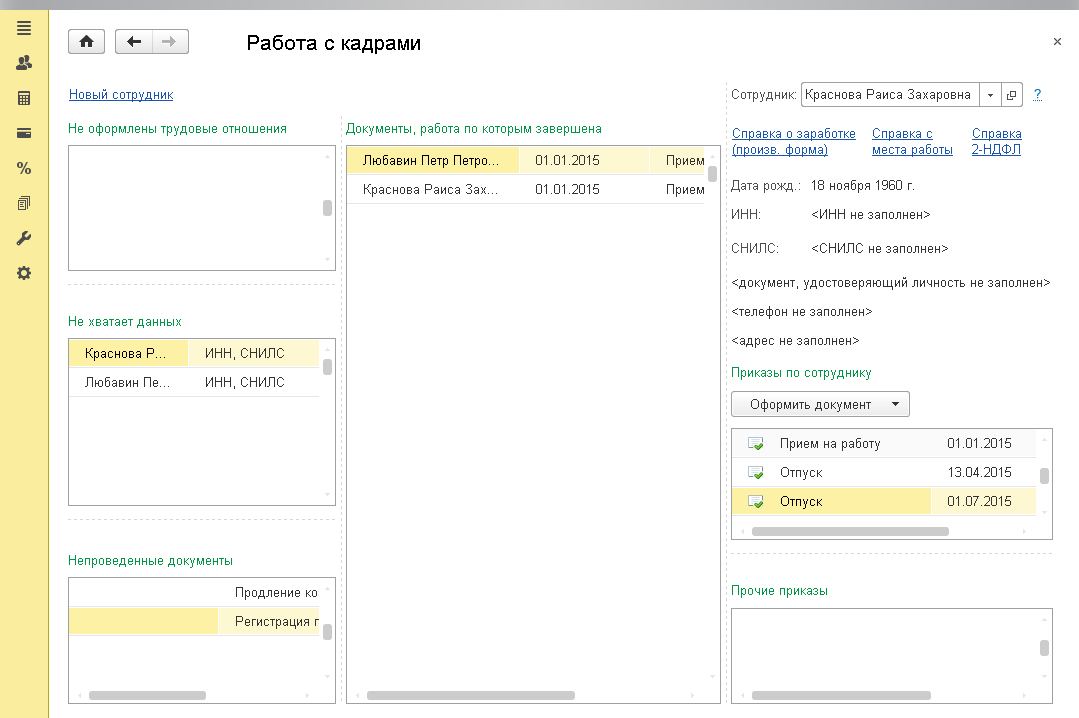
\includegraphics[scale=0.55]{1c_employees.png} 
	\caption{Кадровый учет в системе 1С:Зарплата и управление персоналом}
	\label{fig:analysis:analogues:1c_employees}
\end{figure}

«1С:Зарплата и управление персоналом 8» позволяет:
\begin{itemize}
	\item снизить временные затраты на выполнение кадровой работы;
	\item учитывать движение кадров;
	\item вести учет персональных данных работников;
	\item осуществлять воинский учет;
	\item вести учет рабочего времени;
	\item вести штатное расписание;
\end{itemize}

Преимущества системы:
\begin{itemize}
	\item возможность автоматизации расчета зарплаты;
	\item учет движения кадров;
	\item учет рабочего времени;
	\item возможность учета персональных данных работников.
\end{itemize}

Недостатки системы:
\begin{itemize}
	\item ПО требует приобретения;
	\item устаревший интерфейс;
	\item отсутсвие кроссплатформенности;
	\item сложность использования;
	\item необходимость предварительного обучения персонала.
\end{itemize}
\pagebreak

\subsubsection{} Генерация резюме
\label{sec:analysis:analogues:generation}

В настоящее время практика направления кандидатом, ведущим поиск работы, своего резюме работодателю или компании по
подбору персонала в ответ на его объявление о вакансии находит все большее распространение не только среди
многонациональных, но и беларуских компаний. Представление резюме потенциальному работодателю или агентству по подбору
персонала становится одним из основных методов трудоустройства для квалифицированных кандидатов.

Резюме -- это документ, в котором в краткой, но емкой форме изложены основные сведения о профессиональных умениях и
навыках, трудовой биографии и личных данных кандидата. Оно позволяет работодателю заочно, с минимальными затратами
времени ознакомиться в первом приближении с деловыми и личностными качествами кандидатов, произвести первичный отбор
наиболее достойных и дать первую оценку их соответствия имеющейся вакансии.

Практика показывает, что в большинстве случаев специалист по подбору персонала или менеджер по работе с персоналом при
принятии решения о том, пригласить кандидата на интервью или нет, основывается на содержании и форме резюме \cite{cv}.

Принято считать, что профессионально составленное резюме обычно содержит следующие разделы:
\begin{itemize}
	\item общие данные о кандидате — возраст, адрес проживания, контактная информация;
	\item образование — как основное, так и дополнительное;
	\item профессиональные умения и навыки;
	\item трудовая биография в обратном хронологическом порядке (последнее место работы — сначала);
	\item личные данные о кандидате, его увлечения;
	\item пожелания кандидата относительно будущей должности, уровня компенсации, возможного района или региона работы.
\end{itemize}

Cуществует несколько сервисов, автоматизирующих процесс генерации резюме. В процессе проектирования
системы были изучены следующие существующие аналоги:
\begin{itemize}
	\item cистема генерации резюме CVMaker;
	\item cистема визулизации резюме Vizualize
\end{itemize}

1.2.2.1 Cистема генерации резюме CVMaker

Cистема позволяет пользователям автоматически генерировать резюме(рисунок \ref{fig:analysis:analogues:cvmaker}).
CVMaker дает на выбор 6 бесплатных шаблонов для резюме, выполненных в строгом классическом стиле. Однако система никак
не связана с компанией и не позволяет управлять уже созданными резюме.

Преимущества:
\begin{itemize}
	\item бесплатность;
	\item возможность выбора шаблона;
	\item Возможность выбора формата загрузки.
\end{itemize}

Недостатки:
\begin{itemize}
	\item отсутствие связи с компанией;
	\item невозможность проверки заполненного резюме сотрудником компании встроенными средствами;
	\item невозможность корректировки уже сгенерированного резюме.
\end{itemize}

\begin{figure}[!t]
	\centering
	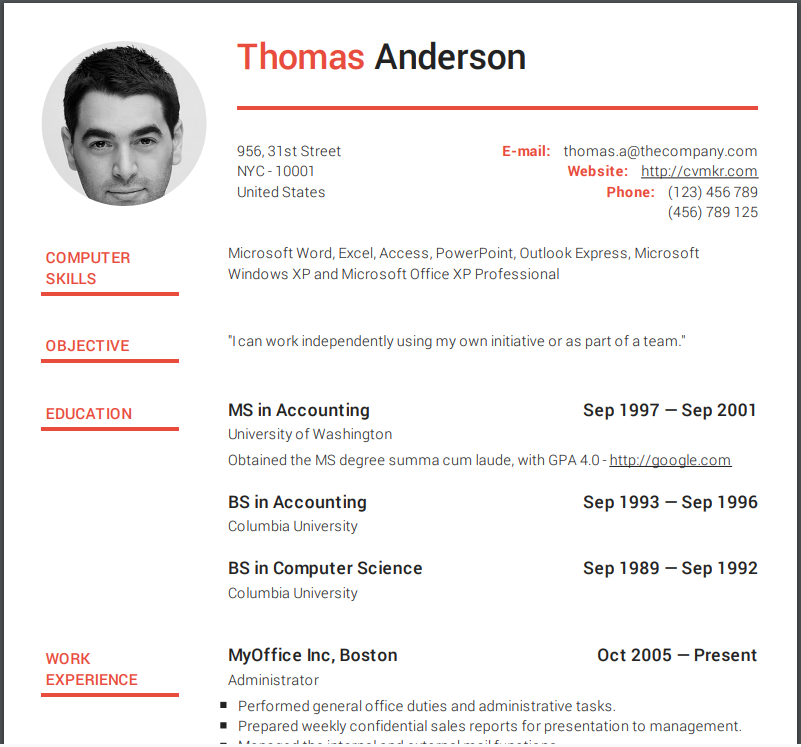
\includegraphics[scale=0.7]{cvmaker.png} 
	\caption{Пример готового резюме в системе СVMaker}
	\label{fig:analysis:analogues:cvmaker}
\end{figure}

1.2.2.2 Cистема визулизации резюме Vizualize

Скучные списки о прошлых местах работы, заслугах и навыках можно превратить в интересную инфографику на
Vizualize(рисунок \ref{fig:analysis:analogues:visualize}). Чтобы создать ее, нужен профиль в LinkedIn. Информацию можно
импортировать также из Twitter, Facebook и Foursquare.

\begin{figure}[!t]
	\centering
	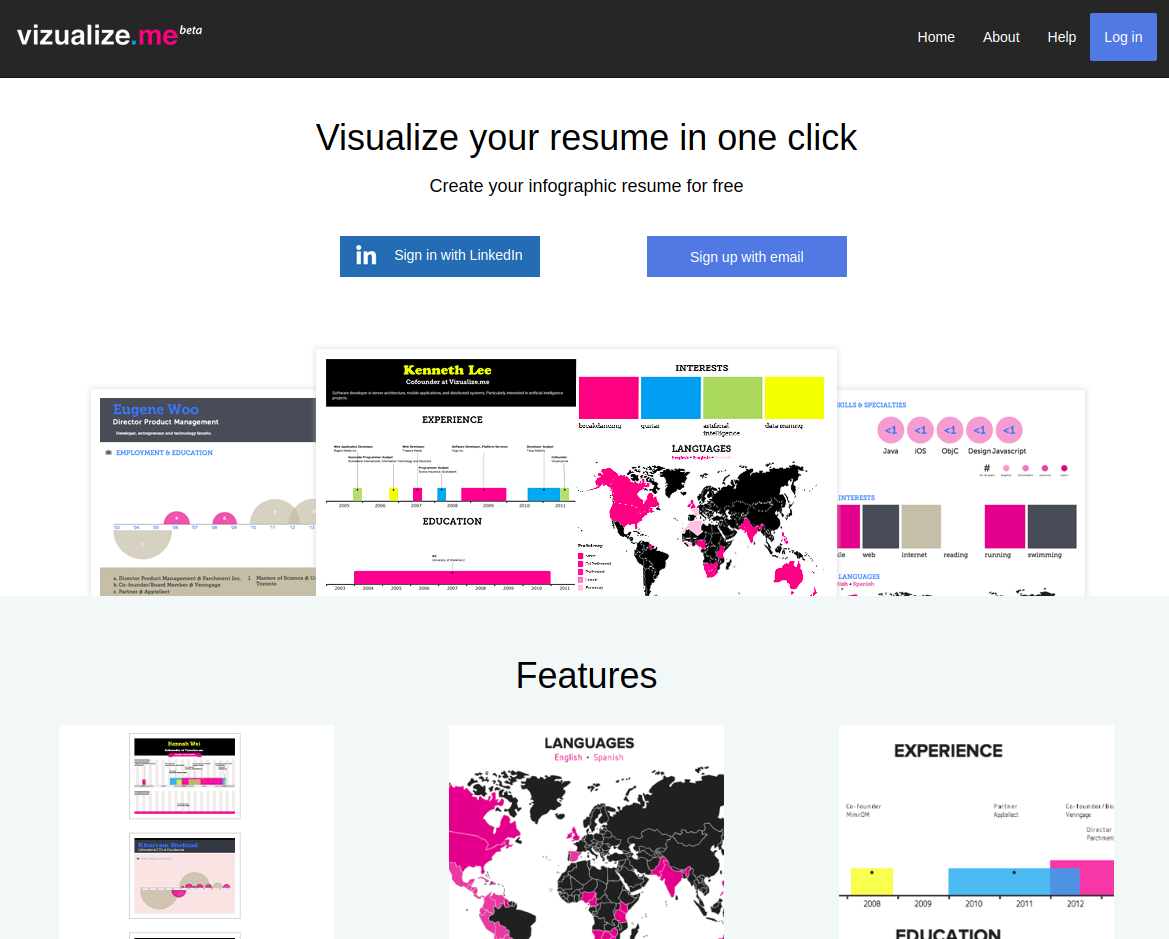
\includegraphics[scale=0.5]{visualize.png} 
	\caption{Стартовая страница Visualize}
	\label{fig:analysis:analogues:visualize}
\end{figure}

Преимущества:
\begin{itemize}
	\item бесплатность;
	\item визуализация резюме;
	\item возможность импорта данных из социальных сетей.
\end{itemize}

Недостатки:
\begin{itemize}
	\item отсутствие связи с компанией;
	\item невозможность проверки заполненного резюме сотрудником компании встроенными средствами;
	\item невозможность вывода резюме на бумажный носитель.
\end{itemize}
